%!TEX root = ../../../tugas-akhir.tex
\section{Evaluasi}
\subsection{Tujuan Pengujian}
Pada penelitian ini pengujian dilakukan untuk melakukan evaluasi apakah modifikasi terhadap perangkat OpenSSL merupakan modifikasi yang baik. Pengujian dilakukan terhadap dua bagian dari OpenSSL, yaitu pengujian terhadap fungsionalitas OpenSSL serta pengujian terhadap kinerja OpenSSL.

Pengujian fungsional dilakukan untuk memastikan bahwa fungsionalitas dari OpenSSL tetap berjalan dengan baik setelah dilakukan modifikasi terhadap \textit{source code}. Pengujian fungsional dilakukan terhadap operasi artimatika big integer yang telah diubah untuk memastikan hasil dari operasi aritmatika tersebut masih merupakan hasil yang benar.

Pengujian kinerja dilakukan untuk menjawab rumusan masalah poin pertama dan ketiga pada subbab \ref{sec:rumusan_masalah}. Pengujian kinerja akan menjawab apakah kinerja TLS dapat meningkat setelah menggunakan algoritma paralel dalam operasi aritmatika big integer. Selain itu, pengujian kinerja akan menunjukkan apakah algoritma paralel yang digunakan dalam operasi aritmatika merupakan algoritma yang tepat atau tidak.

\subsection{Pengujian Fungsional}

\subsubsection{Lingkungan Pengujian}
Lingkungan pengujian yang digunakan dalam pengujian fungsional sama dengan lingkungan implementasi yang telah dijelaskan dalam \ref{sec:impl_env} namun tanpa penggunaan Apache sebagai web server. Pengujian fungsional hanya membutuhkan \textit{source code} OpenSSL serta testcase yang digunakan.

\subsubsection{Skenario Pengujian}
% OpenSSL udah punya tc
OpenSSL telah memiliki kakas yang dapat dilakukan untuk melakukan unit test. Kakas yang digunakan merupakan gabungan dari \textit{perl script} dan kode dalam bahasa C. \textit{Perl script} akan menjalankan kode dalam bahasa C dan memberikan kasus uji yang sesuai untuk pengujian yang dilakukan. Kode dalam bahasa C akan melakukan \textit{parsing} terhadap kasus uji yang ada, menjalakan fungsi tertentu, kemudian mencocokkan hasil dari fungsi tersebut terhadap kasus uji yang diberika.

% jelasin gimana cara run -> makefile
Pengujian fungsional dilakukan melalui makefile dengan command |make test|. Pengujian dilakukan setelah build aplikasi selesai dilakukan, namun sebelum dilakukannya instalasi aplikasi pada sistem. Command |make test| melakukan pengujian terhadap seluruh fungsionalitas OpenSSL, mulai dari library big integer, komputasi kriptografi, sistem sertifikat, serta pembuatan koneksi TLS.

% testcase yang dipilih kayak gimana, kenapa
Kasus uji untuk setiap operasi aritmatika disimpan pada |openssl/test/recipes/10-test_bn_data|. Kasus uji untuk setiap operasi aritmatika memiliki file terpisah dengan operasi artimatika yang lain. Sebagai contoh, kasus uji untuk operasi perkalian disimpan pada file |bnmul.txt| pada direktori pengujian. Contoh kasus uji yang digunakan untuk pengujian fungsional dapat dilihat pada Lampiran \ref{sec:functional_testcase}.

\subsubsection{Hasil Pengujian}
Pengujian fungsionalitas pada OpenSSL berhasil dilakukan. Tidak ada fungsionalitas dari OpenSSL yang rusak setelah dilakukan modifikasi pada \textit{source code} OpenSSL. \textit{Output} dari pengujian fungsional yang dilakukan dapat dilihat pada Lampiran XXX. \todo{tambahin}

\subsection{Pengujian Kinerja}

\subsubsection{Lingkungan Pengujian}

Kakas yang digunakan untuk testing adalah ApacheBench. Sesuai dengan namanya, ApacheBench dapat melakukan benchmarking pada web server. ApacheBench (ab) akan mengirim sejumlah request dan menghasilkan data kinerja web server yang dipilih. Data yang dihasilkan pleh ab diantaranya adalah jumlah byte yang dikirim antar web server dan ab, jumlah request per detik yang dapat ditangani server, waktu rata-rata yang digunakan untuk menangani sebuah request, serta waktu maksimum dan minimum yang digunakan dalam sebuah request.

Pengujian dilakukan pada \textit{cloud provider} DigitalOcean. Cloud dipilih karena proses pembuatan server on-demand dengan spesifikasi tertentu dapat dilakukan dengan mudah dan dalam waktu yang singkat. Penggunaan server dengan jumlah core yang tinggi yang dibutuhkan dapat dilakukan dengan menggunakan DigitalOcean CPU-Optimized Droplet. Droplet tersebut mendapatkan dedicated CPU sehingga komputasi paralel pada OpenSSL dapat berjalan dengan menggunakan CPU pada kapasitas maksimum. Arsitektur yang digunakan pada pengujian dapat dilihat pada Gambar \ref{fig:testing_arch}.

\begin{figure}[h]
  \centering
  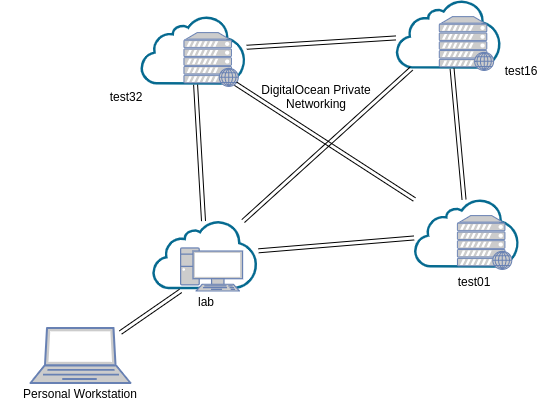
\includegraphics[width=0.8\textwidth]{resources/ch-4/testing_arch.png}
  \caption{Arsitektur Lingkungan Pengujian}
  \label{fig:testing_arch}
\end{figure}

Pengujian menggunakan empat Droplet, yaitu lab, test01, test16, dan test32. Setiap droplet terhubung melalui DigitalOcean Private Networking, dengan demikian latency antar droplet dapat dikurangi hingga seminimum mungkin. Droplet test01, test16, dan test32 merupakan droplet tempat diinstallnya Apache dan OpenSSL. Arsitektur aplikasi yang terinstall pada test01, test16, dan test32 sama dengan arsitektur implementasi pada Gambar \ref{fig:openssl_arch}. Droplet lab digunakan sebagai tempat melakukan testing dan tempat dijalankannya kakas ApacheBench. Komunikasi antar droplet lab dan personal workstation dilakukan dengan ssh. Tabel \ref{tab:droplet_specs} menjelaskan spesifikasi yang dimiliki setiap droplet.

\begin{table}[]
  \caption{Spesifikasi Droplet} % title of Table
  \label{tab:droplet_specs}
  \centering % used for centering table
  \begin{tabular}{@{}rcccc@{}}
\toprule
\multicolumn{1}{c}{\textbf{Spesifikasi}} & \textbf{lab} & \textbf{test01} & \textbf{test16} & \textbf{test32} \\ \midrule
\textbf{vCPU}                            & 1            & 1               & 16              & 32              \\
\textbf{Memori (GB)}                          & 1          & 1             & 32            & 64            \\
\textbf{SSD Disk (GB)}                        & 25         & 25            & 200           & 400           \\ \bottomrule
\end{tabular}
\end{table}

\subsubsection{Skenario Pengujian}
Pengujian dilakukan dengan menjalankan ApacheBench pada node lab dengan tujuan web yang dicek test01, test16, dan test32. ApacheBench menghasilkan beberapa data, namun kita hanya peduli pada data berikut.
% \todo{cite website apachebench}
\begin{enumerate}[label=\roman*.]
  \item \textit{Time taken for tests}, yaitu waktu dari koneksi pertama dibuat sampai response terakhir diterima.
  \item \textit{Requests per second}, yaitu jumlah request yang ditangani dalam satu detik
  \item \textit{Time per request}, yaitu waktu rata-rata untuk sebuah request.
  \item \textit{Min \& max connection times}, yaitu waktu maksimum dan minimum yang digunakan oleh sebuah request.
\end{enumerate}

Pengujian dengan ApacheBench dilakukan terhadap beberapa versi perangkat OpenSSL. Versi pertama adalah OpenSSL vanilla yang belum dimodifikasi, versi kedua adalah OpenSSL dengan paralelisasi modul penjumlahan dan pengurangan, versi ketiga adalah OpenSSL dengan paralelisasi modul perkalian, versi keempat adalah OpenSSL dengan paralelisasi modul pembagian, dan versi kelima adalah OpenSSL dengan semua paralelisasi semua modul operasi aritmatika.

\subsubsection{Hasil dan Analisis Pengujian}

\paragraph{Operasi Penjumlahan}
\begin{figure}
  \centering
  \begin{tikzpicture}
  	\begin{axis}[
  		xlabel=Panjang Data $(bit)$,
  		ylabel={Waktu $(ms)$}
  	]
    \addplot table [x=size, y=c1, col sep=comma] {resources/csv/example.csv};
    \addplot table [x=size, y=c16, col sep=comma] {resources/csv/example.csv};
    \addplot table [x=size, y=c32, col sep=comma] {resources/csv/example.csv};
  	\end{axis}
  \end{tikzpicture}
  \caption{Data Penjumlahan}
  \label{fig:add_data}
\end{figure}

\paragraph{Operasi Pengurangan}
\paragraph{Operasi Perkalian}
\paragraph{Operasi }

  % Langsung data speedup aja, data raw simpen di lampiran
  %
  % \begin{table}[ht]
  % \caption{Test table} % title of Table
  % \centering % used for centering table
  % \begin{tabular}{c c c c} % centered columns (4 columns)
  % \hline\hline %inserts double horizontal lines
  % Case & Method\#1 & Method\#2 & Method\#3 \\ [0.5ex] % inserts table
  % %heading
  % \hline % inserts single horizontal line
  % 1 & 50 & 837 & 970 \\ % inserting body of the table
  % 2 & 47 & 877 & 230 \\
  % 3 & 31 & 25 & 415 \\
  % 4 & 35 & 144 & 2356 \\
  % 5 & 45 & 300 & 556 \\ [1ex] % [1ex] adds vertical space
  % \hline %inserts single line
  % \end{tabular}
  % \label{table:nonlin} % is used to refer this table in the text
  % \end{table}
